\documentclass[10pt]{article}
\usepackage[utf8]{inputenc}
\usepackage[activeacute,spanish]{babel}
\usepackage[left=1.5cm,top=1.5cm,right=1.5cm, bottom=1.5cm,letterpaper, includeheadfoot]{geometry}

\usepackage{amssymb, amsmath, amsthm}
\usepackage{graphicx}
\usepackage{hyperref}
\usepackage{lmodern,url}
\usepackage{paralist} %util para listas compactas
\usepackage{xcolor}
\usepackage{bbm}
\usepackage{mathrsfs}
\usepackage{etaremune}
\usepackage{bbm}

%========PAQUETES AGREGADOS===========
%Pseudocodigo
\usepackage{pseudocode}
\usepackage[portuguese, boxruled]{algorithm2e}
\usepackage{wrapfig}
\usepackage{multicol}
\usepackage{graphicx}
\usepackage{caption}
\usepackage{subcaption}
%\captionsetup[table]{labelformat=empty}
\captionsetup[subfigure]{labelformat=empty}
\usepackage{cancel}
\usepackage{tikz}
\def\checkmark{\tikz\fill[scale=0.4](0,.35) -- (.25,0) -- (1,.7) -- (.25,.15) -- cycle;} 
%====================================

\usepackage{fancyhdr}
\pagestyle{fancy}
\fancypagestyle{plain}{%
\fancyhf{}
\lhead{\footnotesize\itshape\bfseries\rightmark}
\rhead{\footnotesize\itshape\bfseries\leftmark}
}


% macros
\newcommand{\Q}{\mathbb Q}
\newcommand{\R}{\mathbb R}
\newcommand{\N}{\mathbb N}
\newcommand{\Z}{\mathbb Z}
\newcommand{\C}{\mathbb C}
\newcommand{\BigO}{\mathcal{O}}
%Teoremas, Lemas, etc.
\theoremstyle{plain}
\newtheorem{teo}{Teorema}
\newtheorem{lem}{Lema}
\newtheorem{prop}{Proposición}
\newtheorem{cor}{Corolario}
\newtheorem{obs}{Observación}
\newtheorem{ej}{Ejemplo}
\renewcommand{\qedsymbol}{\rule{0.7em}{0.7em}}
\renewenvironment{proof}{{\bfseries \noindent Demostración}}{ \qed \\}


\theoremstyle{definition}
\newtheorem{defi}{Definición}
% fin macros


\newcommand{\catnum}{16} %numero de catedra
\newcommand{\fecha}{13 de Septiembre 2016 }

%%%%%%%%%%%%%%%%%%

%Macros para este documento
\newcommand{\cin}{\operatorname{cint}}



\begin{document}
%Encabezado
\fancyhead[L]{Facultad de Ciencias Físicas y Matemáticas}
\fancyhead[R]{Universidad de Chile}
\vspace*{-1.2 cm}
\begin{minipage}{0.6\textwidth}
\begin{flushleft}
\hspace*{-0.5cm}\textbf{MA3402-1 Estadística. Primavera 2016}\\
\hspace*{-0.5cm}\textbf{Profesor:} Raul Gouet\\
\hspace*{-0.5cm}\textbf{Escriba:} Manuel Cáceres\\
\hspace*{-0.5cm}\textbf{Fecha:} \fecha
\end{flushleft}
\end{minipage}
\begin{minipage}{0.36\textwidth}
\begin{flushright}

\includegraphics[scale=0.3]{imagenes/fcfm_dcc}
\end{flushright}
\end{minipage}
\bigskip
%Fin encabezado

\begin{center}
\LARGE\textbf{Clase \catnum}
\end{center}
Hemos visto las ventajas de contar con modelos que tengan densidades a priori conjugadas, a través de varios ejemplos.\\
El trabajo de cálculo de $\pi(\theta|X)$ se reduce a una actualización de parámetros.
\section{Densidades a priori impropias}
Este es un fenómeno interesante en el que podemos usar como densidad $\pi(\theta)$ a priori una función que no es integrable (sobre $\Theta$), por lo tanto no es densidad de probabilidad.\\

La razón de esto es que una medida positiva (con integral $\infty$) puede reflejar mejor la opinión del analista, que cualquier probabilidad. Además eso conduce a una densidad a posteriori ``legal'', en ocasiones y también, mediante este procedimiento se recuperan algunos resultados de la estadística no bayesiana.\\

Un ejemplo estándar es el caso normal $N(\theta,\sigma^2)$ con $\sigma>0$ conocido $\theta \in \Theta = \mathbb{R}$. Tenemos $X_{1},\ldots,X_{n}$ iid $N(\theta,\sigma^2)$ y definimos $\pi(\theta)0 1  \forall \theta \in \Theta$.\\

Claro que $\int_{\Theta}\pi(\theta)d\theta = \infty$, pero nada impide (formalmente) escribir
\begin{align*}
\pi(\theta|X) &= \frac{f(X|\theta)\pi(\theta)}{f(X)}\\
&= \frac{ke^{-\frac{1}{2\sigma^2}\sum (X_{i}-\theta)^2}\cdot 1}{\int_{-\infty}^{\infty}}f(X|\theta) \underbrace{\pi(\theta)}_{1}d\theta
\end{align*}
La parte de abajo de la fracción
\begin{align*}
k\int_{-\infty}^{\infty}e^{-\frac{1}{2\sigma^2}\sum (X_{i}-\theta)^2}d\theta < \infty ?
\end{align*}
Acomodamos la forma cuadrática
\begin{align*}
-\frac{1}{2\sigma^2}\left(\sum X_{i}^2 - 2n\bar{X}\theta+ n \theta^2\right)\\
-\frac{n}{2\sigma^2}\left(\theta^2-2\bar{X}\theta-\bar{X}^2\right) + R(X)\\
\frac{1}{2\sigma^2/n}(\theta-\bar{X})^2 + R(X)\\
ke^{R(X)}\int_{-\infty}^{\infty}e^{-\frac{1}{2\sigma^2/n}(\theta-\bar{X})^2}d\theta = k e^{R(X)}\sqrt{2\pi}\sigma/\sqrt{n} < \infty
\end{align*}
Dado que $f(X)$ existe tenemos que $\pi(\theta|X)$ es la ley normal $N(\bar{X}, \sigma^2/n)$
\section{Volvamos a los 3 problemas clásicos de los frecuentistas}
\begin{enumerate}
\item Estimación puntual
\item Estimación intervalar o por conjuntos de confianza
\item Test de hipótesis
\end{enumerate}
\textbf{¿Qué hacen los bayesianos enfrentados a estos problemas?}\\

\begin{etaremune}
\item Lo que opina el bayesiano está en $\pi(\theta|X)$. Si tenemos $H_{0}:\theta\in \Theta_{0}$ versus $H_{1}:\theta\in \Theta_{1}$.\\
¿Cómo usar $\pi(\theta|X)$ para decidir (construir un test)?\\

Existe una opinión a priori sobre $H_{0}$ y $H_{1}$(prejuicio)
\begin{align*}
\pi(\Theta_{1}) = \int_{\Theta_{1}}\pi(\theta)d\theta\\
\pi(\Theta_{0}) = \int_{\Theta_{0}}\pi(\theta)d\theta
\end{align*}
Habiendo observado $X=x$, entonces nuestra opinión es:
\begin{align*}
\pi(\Theta_{0}|X) = \int_{\Theta_{0}}\pi(\theta|X)d\theta\\
\pi(\Theta_{1}|X) = \int_{\Theta_{1}}\pi(\theta|X)d\theta
\end{align*}
El test bayesiano entonces es Diga $H_{0}$ si $\pi(\Theta_{0}|X) > \pi(\Theta_{1}|X)$, en caso contrario diga $H_{1}$
\begin{ej}
Calcular el test de Bayes cuando $\Theta = \{\theta_{0},\theta_{1}\}$, es decir, $H_{i}: \theta = \theta_{i}, i = 0,1$.\\
Es este caso $\pi(\theta)$ está caracterizado por $\pi_{0},\pi_{1}(\pi(\theta_{1})$ tales que $\pi_{0}+\pi_{1}=1$ y $\pi(\theta|X) < f(X|\theta)\pi(\theta)$
\end{ej}
\item Con los intervalos de confianza ocurre algo similar (es muy sencillo), lo bayesianos hablan de intervalos de credibilidad.\\
Dado $\alpha \in (0,1)$, buscamos $\theta_{1\alpha}<\theta_{2\alpha}$ tales que (param. real)
\begin{align*}
\mathbb{P}(\theta \in [\theta_{1\alpha}^{(x)},\theta_{2\alpha}^{(x)}]|X) = \int_{\theta_{1\alpha}}^{\theta_{2\alpha}}\pi(\theta|X)dX = 1-\alpha
\end{align*}
\begin{center}
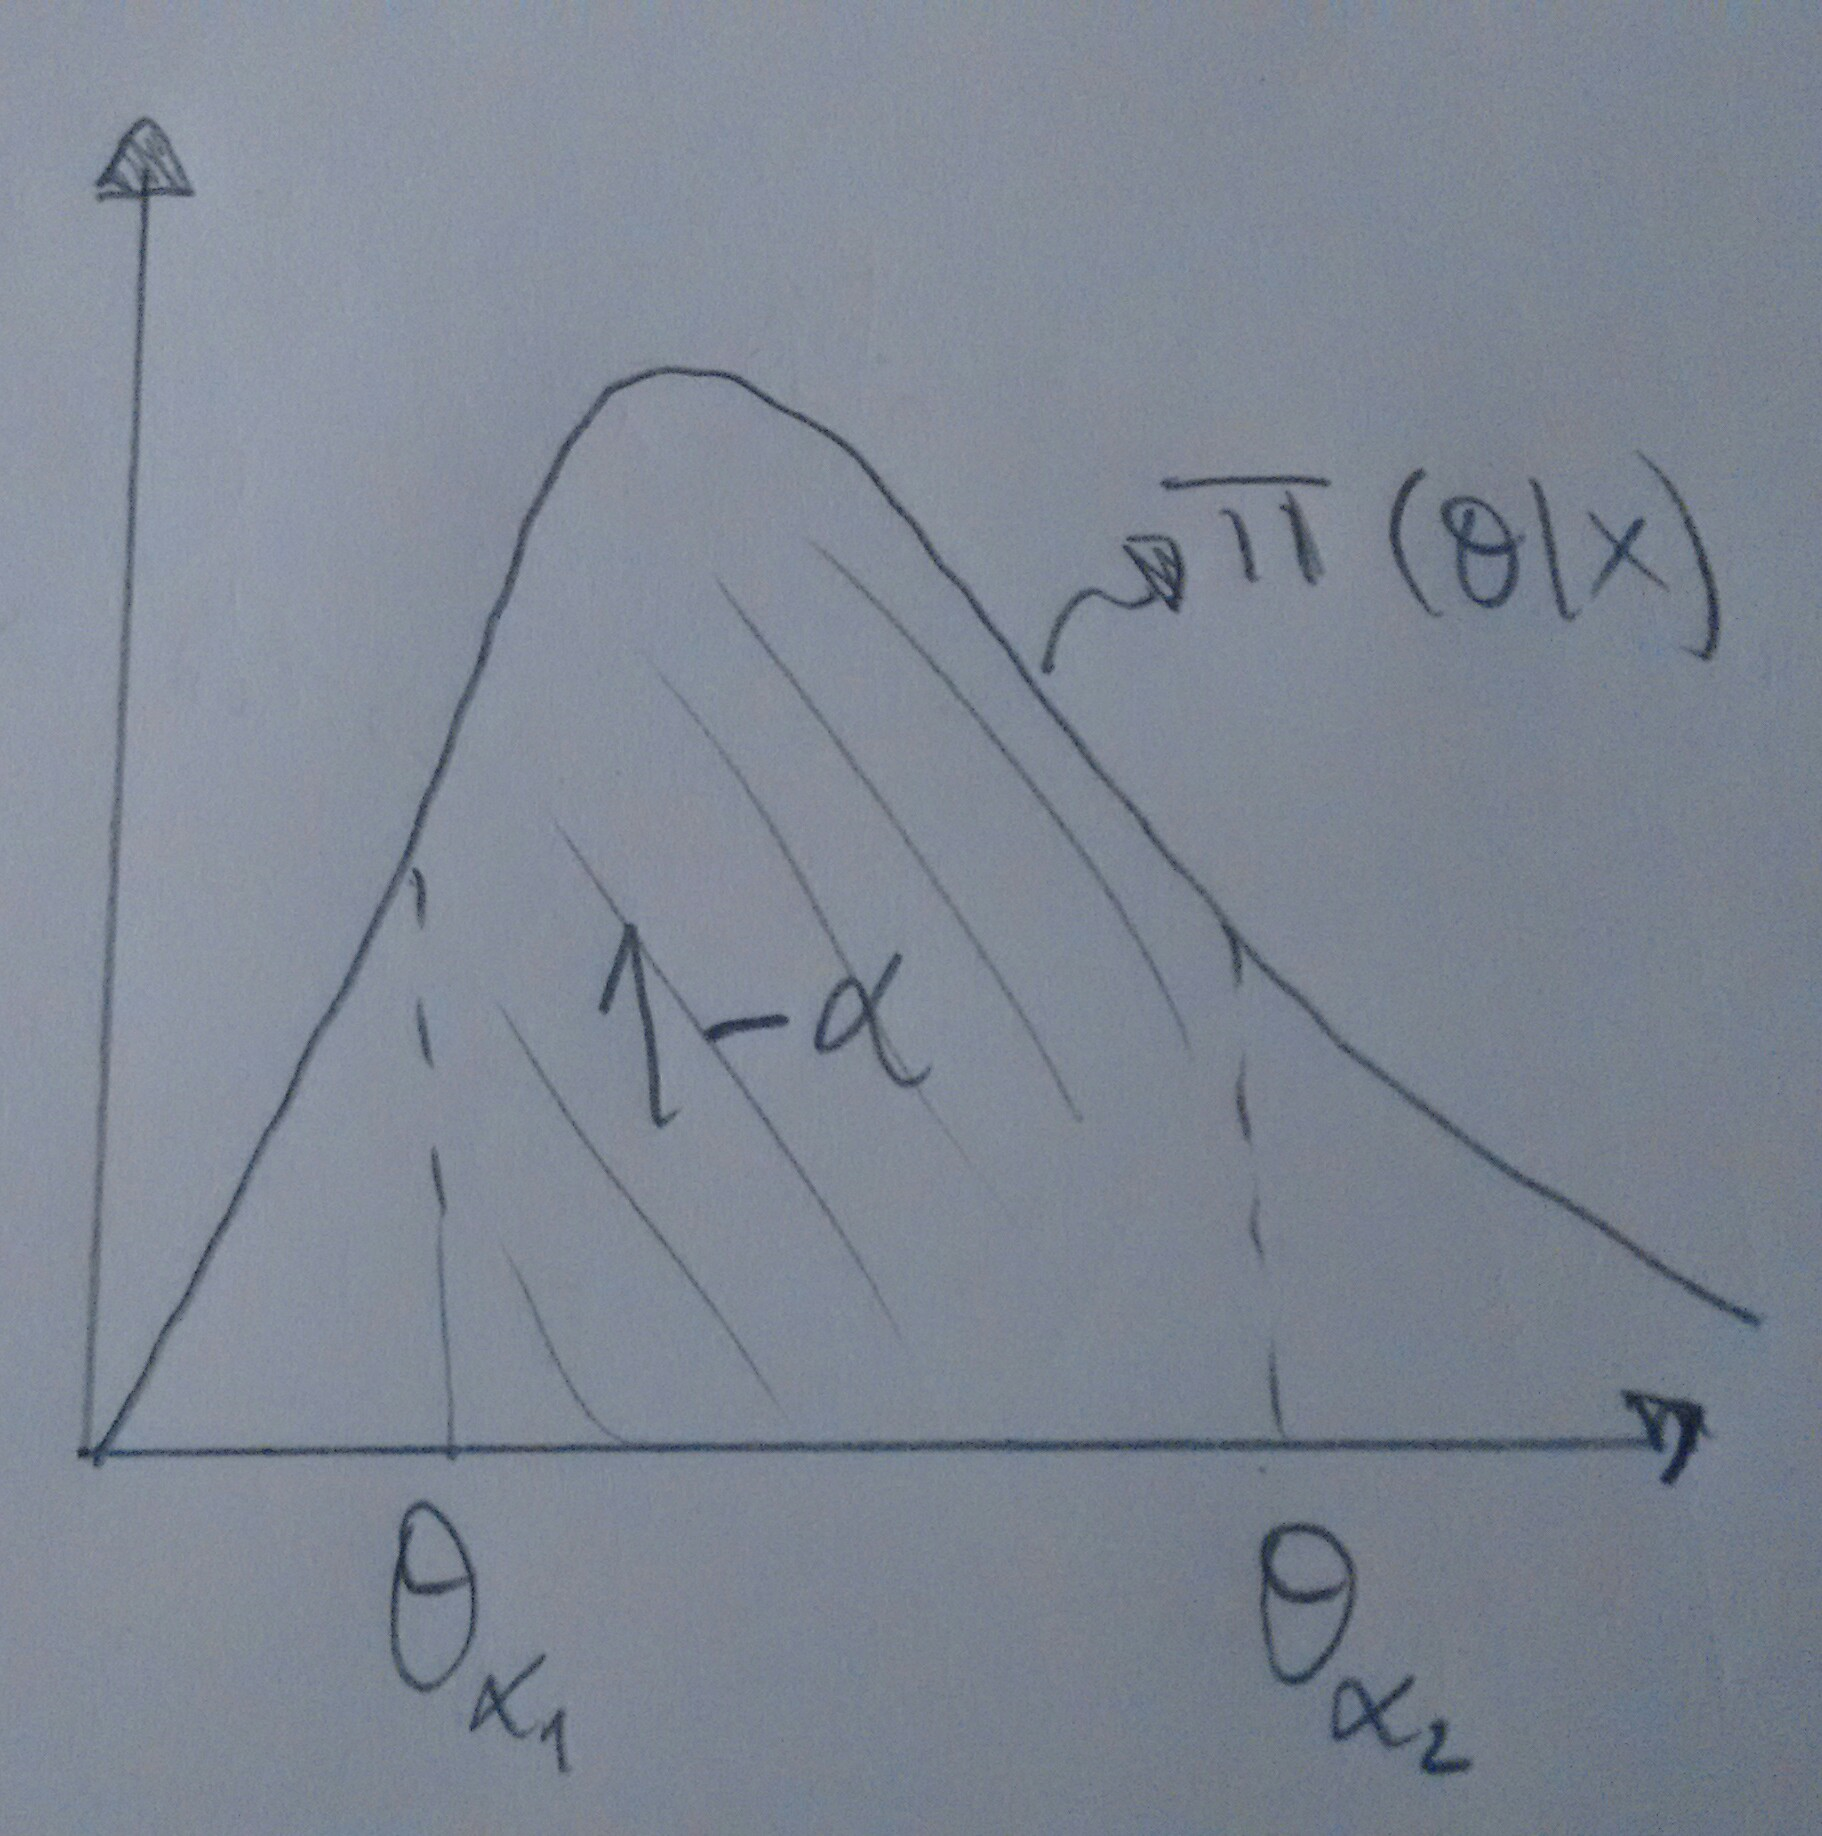
\includegraphics[scale=0.1]{imagenes/credibilidad.jpg}
\end{center}
\item Finalmente volvamos a la estimación puntual, que nos servirá para introducir ideas de teoría de decisiones.\\

Nosotros comenzamos el tema de estimación puntual considerando una función $g(\theta)$ (toda real) que queremos estimar a través de un estimador $\hat{g}(X)$ y usamos el criterio del e.c.m. Calculamos (notación  antigua)
\begin{align*}
ecm_{\theta}(\hat{g}) = \mathbb{E}_{\theta}(\hat{g}(X)-g(\theta))^2
\end{align*}
problema de optimizar el ecm con respecto a $\hat{g}$ (uniforme en $\theta$ (problema variacional).\\

Supongamos que se dispone de $\pi(\theta)$, la densidad a priori. En lugar de buscar óptimos unifrmes en $\theta$, integramos con respecto a $\pi(\theta)$. Es decir, calculamos
\begin{align*}
\underbrace{R(\hat{g})}_{riesgo\ de\ \hat{g}} = \int_{\Theta}ecm_{\theta}(\hat{g}\pi(\theta)d\theta
\end{align*}
Buscamos $\hat{g}$ que minimice el riesgo. esto sigue siendo variacional.\\

Alternativamete podemos intentar resolver el siguiente problema de optimización
\begin{align*}
\min_{\gamma}\int_{\Theta}(\gamma-g(\theta))\pi(\theta|X)d\theta \rightarrow \gamma^{*}(X)
\end{align*}
optimizante, $\mathbb{E}(g(\theta)|X)$, estimador de Bayes de $g(\theta)$.\\

Para terminar tenemos que
\begin{align*}
R(\hat{g}) = \int_{\Theta}\int_{\mathfrak{X}}(\hat{g}(X)-g(\theta))^2f(X|\theta)dx\pi(\theta)d\theta
\end{align*}
usando fubini
\begin{align*}
= \int_{\mathfrak{x}}\int_{\Theta}(\hat{g}(X)-g(\theta))^2\pi(\theta|X)d\theta f(X)dx
\end{align*}
Se observa que $\gamma^*(X) = \mathbb{E}(g(\theta)|X)$ es estimador que minimiza el riesgo $R(\hat{y})$!!
\end{etaremune}
\end{document}